\chapter{方案部署及其效果}
\label{cha:experiment}
本章的主要内容为部署防御方案并验证方案有效性。在真实SDN网络中部署防御方案之后,使用不同形式的LDoS攻击对方案进行测试,探测方案的有效性与开销。

\section{实验准备}
\label{chap5:setup}
本文在真实SDN网络中部署防御系统。防御系统使用的SDN控制器为Floodlight控制器。部署了防御系统的控制器被部署在一个服务器上,该服务器的配置为Intel Xeon Quad-Core CPU E5504和4GB的RAM。在系统中我们使用了OpenFlow商业硬件交换机(EdgeCore AS4610-54T)作为真实SDN网络使用的硬件交换机。硬件交换机的端口转发速率最高能够可达到1Gbps,本文将最大转发速率标记为$R_m$。为了验证系统有效性,本文使用C代码生成不同$T$与$L$的LDoS攻击。并且使用Python代码完成分布式LDoS攻击的部署。

图\ref{fig:topology}展示了实验使用的SDN网络拓扑图。它有7个主机和3个OpenFlow硬件交换机组成。其中2个主机为攻击主机,5个主机为正常的主机。在实验中,$h_1$与$h_5$之间建立TCP连接,$h_3$发送正常流量作为背景流量并由$h_6$接收。$h_2$和$h_4$被设置为LDoS攻击的发送端,由$h_7$接收他们发送的LDoS攻击流量。对于攻击者$h_2$和$h_4$的不同配置可以得到单一攻击源的LDoS攻击,也可以得到分布式LDoS攻击。

%对于这个网络,LDoS攻击流的目的是完全占用$S_2$与$S_3$之间连接的带宽致使$S_2$的队列被拥塞造成$h_1$

\begin{figure}
    \centering
    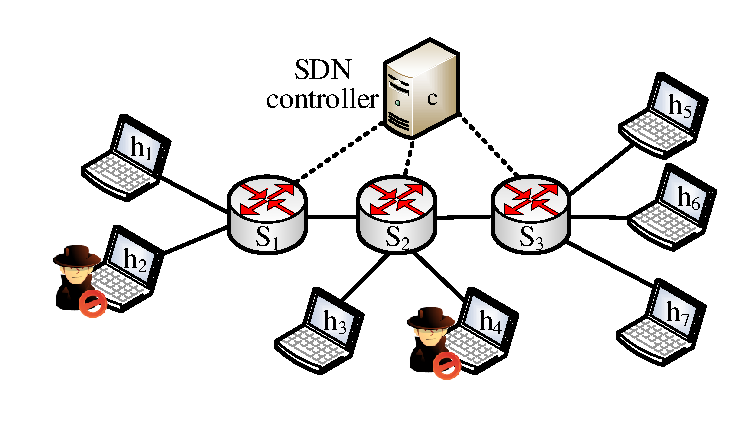
\includegraphics[scale=1]{topology}
    \caption{实验使用拓扑图}
    \label{fig:topology}
\end{figure}

\section{LDoS防御系统结果分析}
\label{chap5:resultanalysis}

\subsection{}

\section{攻击限制策略方案}